\newpage
\chapter{剽窃代码收集区}
\thispagestyle{chapterpage}

这个章节主要存放一些从网上剽窃的代码,诸如\href{https://www.zhihu.com/}{知乎},\href{https://tex.stackexchange.com/}{stackexchange}……我会尽量注明代码来源,如果读者要用这些代码,也请注明原始来源,以示尊重,谢谢合作。

\section{\LaTeX{}实现类似中括号的方框}

\note[方案1]{\href{https://www.zhihu.com/question/55702781}{\LaTeX{}如何实现类似于中括号的方框?-知乎}}

\begin{latex}
\documentclass{article}
\usepackage{tcolorbox}
\tcbuselibrary{most}
\usepackage{lipsum}

\newtcolorbox{mybox}{%
    freelance,
    breakable,
frame code={%
    \draw[line width = 2pt]
    ([xshift=0.5cm]frame.north west) --
    (frame.north west) --
    (frame.south west) --
    ([xshift=0.5cm]frame.south west);
    \draw[line width = 2pt]
    ([xshift=-0.5cm]frame.north east) --
    (frame.north east) --
    (frame.south east) --
    ([xshift=-0.5cm]frame.south east);
},
    colback=white
}

\begin{document}
\lipsum[4]
\begin{mybox}
\lipsum[4]
\end{mybox}
\lipsum[4]
\end{document}
\end{latex}

效果如\autoref{fig:plagiarism-braketbox1}~所示:

\begin{figure}[tbph!]
    \centering
    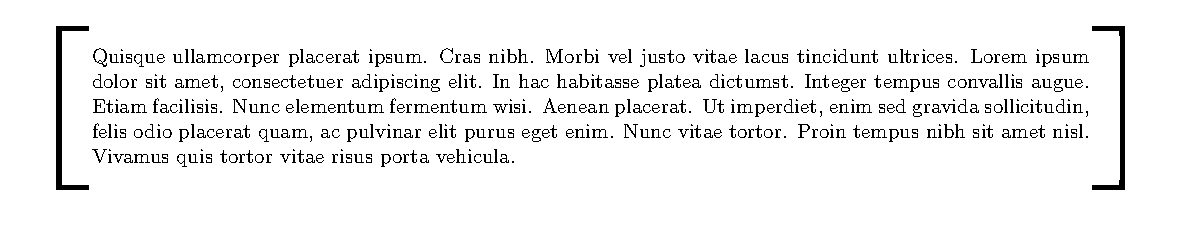
\includegraphics[width=0.8\linewidth]{plagiarism-braketbox1}
    \caption{\LaTeX{}实现类似中括号的方框}
    \label{fig:plagiarism-braketbox1}
\end{figure}

\note[方案2]{\href{http://www.latexstudio.net/archives/9522}{如何实现类似于中括号的方框提示框-\LaTeX{}工作室}}

\begin{latex}
\documentclass[UTF8, openany,twoside]{ctexbook}

\usepackage[tikz]{bclogo,rotating}
\usepackage{tikz}
\usepackage{mdframed}
\usepackage{geometry}
\usepackage{graphicx}
\usetikzlibrary{calc}
\DeclareGraphicsRule{.mps}{eps}{.mps}{}

\geometry{left=2.5cm,right=2.5cm,top=2.5cm,bottom=2.5cm}

\newenvironment{attention}[1]
{\par\medskip\noindent
    \begin{tikzpicture}
    \node[inner sep = 0pt] (box) \bgroup%
    \begin{minipage}[t]{.99\textwidth}%
    \begin{minipage}{.3\textwidth}
    \centering
    \tikz[scale = 5]\node[scale = 3, rotate = 30]{\bclampe};
    \end{minipage}%
    \begin{minipage}{.65\textwidth}
    \textbf{#1}\par\smallskip
    \surroundwithmdframed
    [topline=false, bottomline=false, leftline=false, rightline=false,
    backgroundcolor=lbcolor]
    {minted}}% former part
{%
    \end{minipage}\hfill
    \end{minipage}%
    \egroup;
    \draw[black,line width=3pt]
    ( $ (box.north east) + (-5pt,3pt) $ ) -- ( $ (box.north east) + (0,3pt) $ ) -- ( $ (box.south east) + (0,-3pt) $ ) -- + (-5pt,0);
    \draw[black,line width=3pt]
    ( $ (box.north west) + (5pt,3pt) $ ) -- ( $ (box.north west) + (0,3pt) $ ) -- ( $ (box.south west) + (0,-3pt) $ ) -- + (5pt,0);
    \end{tikzpicture}
    \par\medskip}

\begin{document}
    \begin{attention}{Attention}
        如何用 LaTeX 实现这种方框, 要求方框的高度能够随着中间内容的多少自动调整.
    \end{attention}
\end{document}
\end{latex}

效果如\autoref{fig:plagiarism-braketbox2}~所示:

\begin{figure}[tbph!]
    \centering
    
\includegraphics[width=0.8\linewidth]{plagiarism-braketbox2}
    \caption{\LaTeX{}实现类似中括号的方框}
    \label{fig:plagiarism-braketbox2}
\end{figure}

\section{脚注的带圈数字解决方案}

\note[来源]{\href{https://www.zhihu.com/question/29557216}{\TeX{}的脚注怎么设置比较合理?-知乎}}

\LaTeX{}默认的脚注是上标数字,如果对字母或数字进行脚注解释,很容易背误解为「幂」,如P$ ^1 $,42$ ^2 $。关于带圈数字有不少解决方案,目前我用得比较舒服的是重庆大学毕业论文模版里的方法\footnote{\href{https://github.com/nanmu42/CQUThesis}{GitHub - nanmu42/CQUThesis: 重庆大学毕业论文LaTeX模板}},优点是带圈数字和\lstinline|\rmfamily|字体一致,但是数字不能超过10。

这里提供的刘海洋的解决方法,数字可以超过10,但是带圈数字字体由ipag.ttf提供,与罗马字族字体不一致。对中文文档,xeCJK将20以内的带圈数字认做西文符号,20以上的带圈数字认做CJK符号,因此需要分别设置字体(或者改变这些符号的类型)。

\begin{latex}
\usepackage{xunicode-addon}
\newfontfamily\fnmarkfont{ipag.ttf} % 带圈 0 到 20 被认做西文符号
\newCJKfontfamily\fnCJKmarkfont{ipag.ttf} % 带圈数字超过 20 是 CJK 符号
\renewcommand\thefootnote{{\fnmarkfont\fnCJKmarkfont\textcircled{\arabic{footnote}}}}
\end{latex}

效果如\autoref{fig:plagiarism-footnote}~所示:

\begin{figure}[!htbp]
    \centering
    \fbox{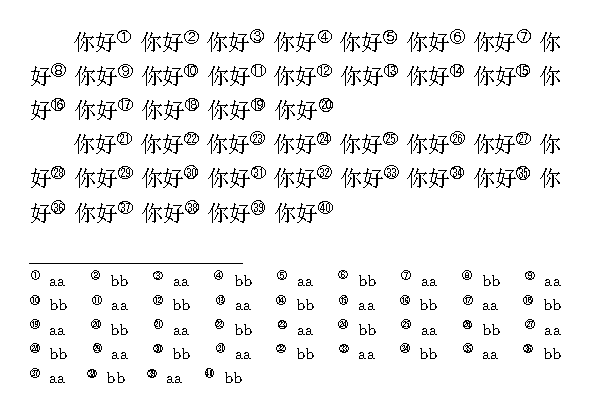
\includegraphics[width=0.8\linewidth]{plagiarism-footnote}}
    \caption{带圈脚注示意图}
    \label{fig:plagiarism-footnote}
\end{figure}

\section{自用的旧的titlesec设置}

\begin{latex}
\titleformat{\chapter}[hang]%
    {\centering\color{title}\heiti\zihao{1}}%格式
    {}
%    {第\, \thechapter 节}%标签
    {20pt}%标签和标题间距
    {}%
    [\vspace{5mm}]%
\titleformat{\section}[hang]%
    {\color{title}\heiti\zihao{-4}}%
    {\thesection.}%
    {5pt}%
    {}%
    []%
\titleformat{\subsection}[hang]%
    {\color{title}\heiti\zihao{-4}}%
    {\thesubsection.}%
    {5pt}%
    {}%
    []%
\titlespacing{\chapter}{0pt}{0pt}{0pt}
\titlespacing{\section}{0pt}{0pt}{0pt}
\titlespacing{\subsection}{0pt}{0pt}{0pt}
\end{latex}



